% !TEX root = main.tex
\section{Auswertung Milchstrasse}
\begin{figure}[H]
    \centering
    % GNUPLOT: LaTeX picture with Postscript
\begingroup
  % Encoding inside the plot.  In the header of your document, this encoding
  % should to defined, e.g., by using
  % \usepackage[cp1252,<other encodings>]{inputenc}
  \inputencoding{cp1252}%
  \makeatletter
  \providecommand\color[2][]{%
    \GenericError{(gnuplot) \space\space\space\@spaces}{%
      Package color not loaded in conjunction with
      terminal option `colourtext'%
    }{See the gnuplot documentation for explanation.%
    }{Either use 'blacktext' in gnuplot or load the package
      color.sty in LaTeX.}%
    \renewcommand\color[2][]{}%
  }%
  \providecommand\includegraphics[2][]{%
    \GenericError{(gnuplot) \space\space\space\@spaces}{%
      Package graphicx or graphics not loaded%
    }{See the gnuplot documentation for explanation.%
    }{The gnuplot epslatex terminal needs graphicx.sty or graphics.sty.}%
    \renewcommand\includegraphics[2][]{}%
  }%
  \providecommand\rotatebox[2]{#2}%
  \@ifundefined{ifGPcolor}{%
    \newif\ifGPcolor
    \GPcolorfalse
  }{}%
  \@ifundefined{ifGPblacktext}{%
    \newif\ifGPblacktext
    \GPblacktexttrue
  }{}%
  % define a \g@addto@macro without @ in the name:
  \let\gplgaddtomacro\g@addto@macro
  % define empty templates for all commands taking text:
  \gdef\gplbacktext{}%
  \gdef\gplfronttext{}%
  \makeatother
  \ifGPblacktext
    % no textcolor at all
    \def\colorrgb#1{}%
    \def\colorgray#1{}%
  \else
    % gray or color?
    \ifGPcolor
      \def\colorrgb#1{\color[rgb]{#1}}%
      \def\colorgray#1{\color[gray]{#1}}%
      \expandafter\def\csname LTw\endcsname{\color{white}}%
      \expandafter\def\csname LTb\endcsname{\color{black}}%
      \expandafter\def\csname LTa\endcsname{\color{black}}%
      \expandafter\def\csname LT0\endcsname{\color[rgb]{1,0,0}}%
      \expandafter\def\csname LT1\endcsname{\color[rgb]{0,1,0}}%
      \expandafter\def\csname LT2\endcsname{\color[rgb]{0,0,1}}%
      \expandafter\def\csname LT3\endcsname{\color[rgb]{1,0,1}}%
      \expandafter\def\csname LT4\endcsname{\color[rgb]{0,1,1}}%
      \expandafter\def\csname LT5\endcsname{\color[rgb]{1,1,0}}%
      \expandafter\def\csname LT6\endcsname{\color[rgb]{0,0,0}}%
      \expandafter\def\csname LT7\endcsname{\color[rgb]{1,0.3,0}}%
      \expandafter\def\csname LT8\endcsname{\color[rgb]{0.5,0.5,0.5}}%
    \else
      % gray
      \def\colorrgb#1{\color{black}}%
      \def\colorgray#1{\color[gray]{#1}}%
      \expandafter\def\csname LTw\endcsname{\color{white}}%
      \expandafter\def\csname LTb\endcsname{\color{black}}%
      \expandafter\def\csname LTa\endcsname{\color{black}}%
      \expandafter\def\csname LT0\endcsname{\color{black}}%
      \expandafter\def\csname LT1\endcsname{\color{black}}%
      \expandafter\def\csname LT2\endcsname{\color{black}}%
      \expandafter\def\csname LT3\endcsname{\color{black}}%
      \expandafter\def\csname LT4\endcsname{\color{black}}%
      \expandafter\def\csname LT5\endcsname{\color{black}}%
      \expandafter\def\csname LT6\endcsname{\color{black}}%
      \expandafter\def\csname LT7\endcsname{\color{black}}%
      \expandafter\def\csname LT8\endcsname{\color{black}}%
    \fi
  \fi
    \setlength{\unitlength}{0.0500bp}%
    \ifx\gptboxheight\undefined%
      \newlength{\gptboxheight}%
      \newlength{\gptboxwidth}%
      \newsavebox{\gptboxtext}%
    \fi%
    \setlength{\fboxrule}{0.5pt}%
    \setlength{\fboxsep}{1pt}%
\begin{picture}(7200.00,5040.00)%
    \gplgaddtomacro\gplbacktext{%
      \csname LTb\endcsname%%
      \put(814,704){\makebox(0,0)[r]{\strut{}$-30$}}%
      \put(814,1161){\makebox(0,0)[r]{\strut{}$-20$}}%
      \put(814,1618){\makebox(0,0)[r]{\strut{}$-10$}}%
      \put(814,2076){\makebox(0,0)[r]{\strut{}$0$}}%
      \put(814,2533){\makebox(0,0)[r]{\strut{}$10$}}%
      \put(814,2990){\makebox(0,0)[r]{\strut{}$20$}}%
      \put(814,3447){\makebox(0,0)[r]{\strut{}$30$}}%
      \put(814,3905){\makebox(0,0)[r]{\strut{}$40$}}%
      \put(814,4362){\makebox(0,0)[r]{\strut{}$50$}}%
      \put(814,4819){\makebox(0,0)[r]{\strut{}$60$}}%
      \put(1278,484){\makebox(0,0){\strut{}$-200$}}%
      \put(2383,484){\makebox(0,0){\strut{}$-100$}}%
      \put(3488,484){\makebox(0,0){\strut{}$0$}}%
      \put(4593,484){\makebox(0,0){\strut{}$100$}}%
      \put(5698,484){\makebox(0,0){\strut{}$200$}}%
      \put(6803,484){\makebox(0,0){\strut{}$300$}}%
    }%
    \gplgaddtomacro\gplfronttext{%
      \csname LTb\endcsname%%
      \put(209,2761){\rotatebox{-270}{\makebox(0,0){\strut{}temperature in $\si{}{K}$}}}%
      \put(3874,154){\makebox(0,0){\strut{}velocity relative to LSR in $\si{}{\frac{km}{s}}$}}%
      \csname LTb\endcsname%%
      \put(5816,4646){\makebox(0,0)[r]{\strut{}$\si{1}{s}$}}%
      \csname LTb\endcsname%%
      \put(5816,4426){\makebox(0,0)[r]{\strut{}$\si{3}{s}$}}%
      \csname LTb\endcsname%%
      \put(5816,4206){\makebox(0,0)[r]{\strut{}$\si{10}{s}$}}%
      \csname LTb\endcsname%%
      \put(5816,3986){\makebox(0,0)[r]{\strut{}$\si{30}{s}$}}%
      \csname LTb\endcsname%%
      \put(5816,3766){\makebox(0,0)[r]{\strut{}$\si{100}{s}$}}%
      \csname LTb\endcsname%%
      \put(5816,3546){\makebox(0,0)[r]{\strut{}$\si{300}{s}$}}%
    }%
    \gplbacktext
    \put(0,0){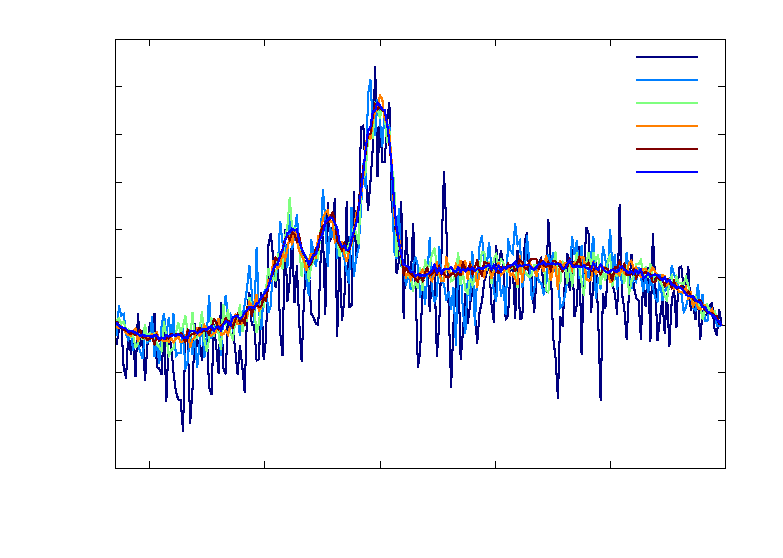
\includegraphics{plots/Belichtungszeit}}%
    \gplfronttext
  \end{picture}%
\endgroup
   
    \caption[Gemessenen Spektren bei verschiedenen Belichtungszeiten]{Mithilfe dieser Abbildung lässt sich erkennen wie sich die gemessenen Spektren mit der Belichtungszeit verändern. Bei einer Belichtungszeit von \SI{1}{s} ist ein sehr ausgeprägtes Rauschen des Signals zu verzeichnen. Maxima sind bei dieser Belichtungszeit kaum ausmachbar. Das Rauschen ist allerdings schon bei einer Belichtungszeit von \SI{10}{s} deutlich reduziert ausgeprägt. Maxima lassen sich bei dieser Belichtungszeit deutlich genauer ausmachen.}
    \label{fig:Belichtungszeit}
\end{figure}

\begin{figure}[H]
    \centering
    % GNUPLOT: LaTeX picture with Postscript
\begingroup
  % Encoding inside the plot.  In the header of your document, this encoding
  % should to defined, e.g., by using
  % \usepackage[cp1252,<other encodings>]{inputenc}
  \inputencoding{cp1252}%
  \makeatletter
  \providecommand\color[2][]{%
    \GenericError{(gnuplot) \space\space\space\@spaces}{%
      Package color not loaded in conjunction with
      terminal option `colourtext'%
    }{See the gnuplot documentation for explanation.%
    }{Either use 'blacktext' in gnuplot or load the package
      color.sty in LaTeX.}%
    \renewcommand\color[2][]{}%
  }%
  \providecommand\includegraphics[2][]{%
    \GenericError{(gnuplot) \space\space\space\@spaces}{%
      Package graphicx or graphics not loaded%
    }{See the gnuplot documentation for explanation.%
    }{The gnuplot epslatex terminal needs graphicx.sty or graphics.sty.}%
    \renewcommand\includegraphics[2][]{}%
  }%
  \providecommand\rotatebox[2]{#2}%
  \@ifundefined{ifGPcolor}{%
    \newif\ifGPcolor
    \GPcolorfalse
  }{}%
  \@ifundefined{ifGPblacktext}{%
    \newif\ifGPblacktext
    \GPblacktexttrue
  }{}%
  % define a \g@addto@macro without @ in the name:
  \let\gplgaddtomacro\g@addto@macro
  % define empty templates for all commands taking text:
  \gdef\gplbacktext{}%
  \gdef\gplfronttext{}%
  \makeatother
  \ifGPblacktext
    % no textcolor at all
    \def\colorrgb#1{}%
    \def\colorgray#1{}%
  \else
    % gray or color?
    \ifGPcolor
      \def\colorrgb#1{\color[rgb]{#1}}%
      \def\colorgray#1{\color[gray]{#1}}%
      \expandafter\def\csname LTw\endcsname{\color{white}}%
      \expandafter\def\csname LTb\endcsname{\color{black}}%
      \expandafter\def\csname LTa\endcsname{\color{black}}%
      \expandafter\def\csname LT0\endcsname{\color[rgb]{1,0,0}}%
      \expandafter\def\csname LT1\endcsname{\color[rgb]{0,1,0}}%
      \expandafter\def\csname LT2\endcsname{\color[rgb]{0,0,1}}%
      \expandafter\def\csname LT3\endcsname{\color[rgb]{1,0,1}}%
      \expandafter\def\csname LT4\endcsname{\color[rgb]{0,1,1}}%
      \expandafter\def\csname LT5\endcsname{\color[rgb]{1,1,0}}%
      \expandafter\def\csname LT6\endcsname{\color[rgb]{0,0,0}}%
      \expandafter\def\csname LT7\endcsname{\color[rgb]{1,0.3,0}}%
      \expandafter\def\csname LT8\endcsname{\color[rgb]{0.5,0.5,0.5}}%
    \else
      % gray
      \def\colorrgb#1{\color{black}}%
      \def\colorgray#1{\color[gray]{#1}}%
      \expandafter\def\csname LTw\endcsname{\color{white}}%
      \expandafter\def\csname LTb\endcsname{\color{black}}%
      \expandafter\def\csname LTa\endcsname{\color{black}}%
      \expandafter\def\csname LT0\endcsname{\color{black}}%
      \expandafter\def\csname LT1\endcsname{\color{black}}%
      \expandafter\def\csname LT2\endcsname{\color{black}}%
      \expandafter\def\csname LT3\endcsname{\color{black}}%
      \expandafter\def\csname LT4\endcsname{\color{black}}%
      \expandafter\def\csname LT5\endcsname{\color{black}}%
      \expandafter\def\csname LT6\endcsname{\color{black}}%
      \expandafter\def\csname LT7\endcsname{\color{black}}%
      \expandafter\def\csname LT8\endcsname{\color{black}}%
    \fi
  \fi
    \setlength{\unitlength}{0.0500bp}%
    \ifx\gptboxheight\undefined%
      \newlength{\gptboxheight}%
      \newlength{\gptboxwidth}%
      \newsavebox{\gptboxtext}%
    \fi%
    \setlength{\fboxrule}{0.5pt}%
    \setlength{\fboxsep}{1pt}%
\begin{picture}(7200.00,5040.00)%
    \gplgaddtomacro\gplbacktext{%
      \csname LTb\endcsname%%
      \put(814,704){\makebox(0,0)[r]{\strut{}$-30$}}%
      \put(814,1161){\makebox(0,0)[r]{\strut{}$-20$}}%
      \put(814,1618){\makebox(0,0)[r]{\strut{}$-10$}}%
      \put(814,2076){\makebox(0,0)[r]{\strut{}$0$}}%
      \put(814,2533){\makebox(0,0)[r]{\strut{}$10$}}%
      \put(814,2990){\makebox(0,0)[r]{\strut{}$20$}}%
      \put(814,3447){\makebox(0,0)[r]{\strut{}$30$}}%
      \put(814,3905){\makebox(0,0)[r]{\strut{}$40$}}%
      \put(814,4362){\makebox(0,0)[r]{\strut{}$50$}}%
      \put(814,4819){\makebox(0,0)[r]{\strut{}$60$}}%
      \put(1278,484){\makebox(0,0){\strut{}$-200$}}%
      \put(2383,484){\makebox(0,0){\strut{}$-100$}}%
      \put(3488,484){\makebox(0,0){\strut{}$0$}}%
      \put(4593,484){\makebox(0,0){\strut{}$100$}}%
      \put(5698,484){\makebox(0,0){\strut{}$200$}}%
      \put(6803,484){\makebox(0,0){\strut{}$300$}}%
    }%
    \gplgaddtomacro\gplfronttext{%
      \csname LTb\endcsname%%
      \put(209,2761){\rotatebox{-270}{\makebox(0,0){\strut{}Temperatur in $\si{}{K}$}}}%
      \put(3874,154){\makebox(0,0){\strut{}velocity relative to LSR in $\si{}{\frac{km}{s}}$}}%
      \csname LTb\endcsname%%
      \put(5816,4646){\makebox(0,0)[r]{\strut{}$\si{1}{s}$}}%
      \csname LTb\endcsname%%
      \put(5816,4426){\makebox(0,0)[r]{\strut{}$\si{30}{s}$}}%
      \csname LTb\endcsname%%
      \put(5816,4206){\makebox(0,0)[r]{\strut{}$\si{300}{s}$}}%
    }%
    \gplbacktext
    \put(0,0){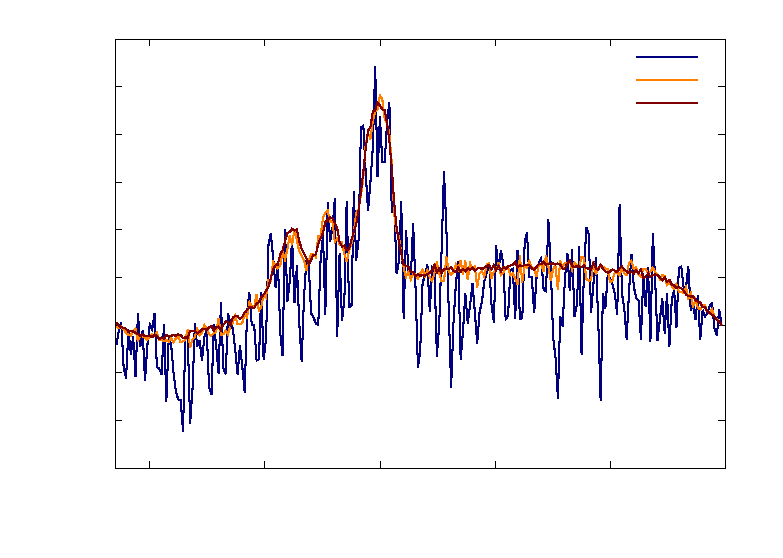
\includegraphics{plots/BelichtungszeitExtrema}}%
    \gplfronttext
  \end{picture}%
\endgroup
   
    \caption[Eindeutigen Unterschiede der Spektren bei verschiedenen Belichtungszeiten]{Diese Abbildung soll noch einmal die eindeutigen Unterschiede der Spektren bei verschiedenen Belichtungszeiten verdeutlichen. Da sich das Spektrum bei einer Belichtungszeit von \SI{30}{s} und \SI{300}{s} nur noch minimal unterscheidet. Haben wir eine Belichtungszeit für unsere Spektren von \SI{60}{s} gewählt. Bei dieser Zeit sind alle Maxima deutlich ausmachbar und der zeitlich begrenzte Versuchszeitraum wird nicht gesprengt.}
    \label{fig:BelichtungszeitExtremal}
\end{figure}

\begin{figure}[H]
    \centering
    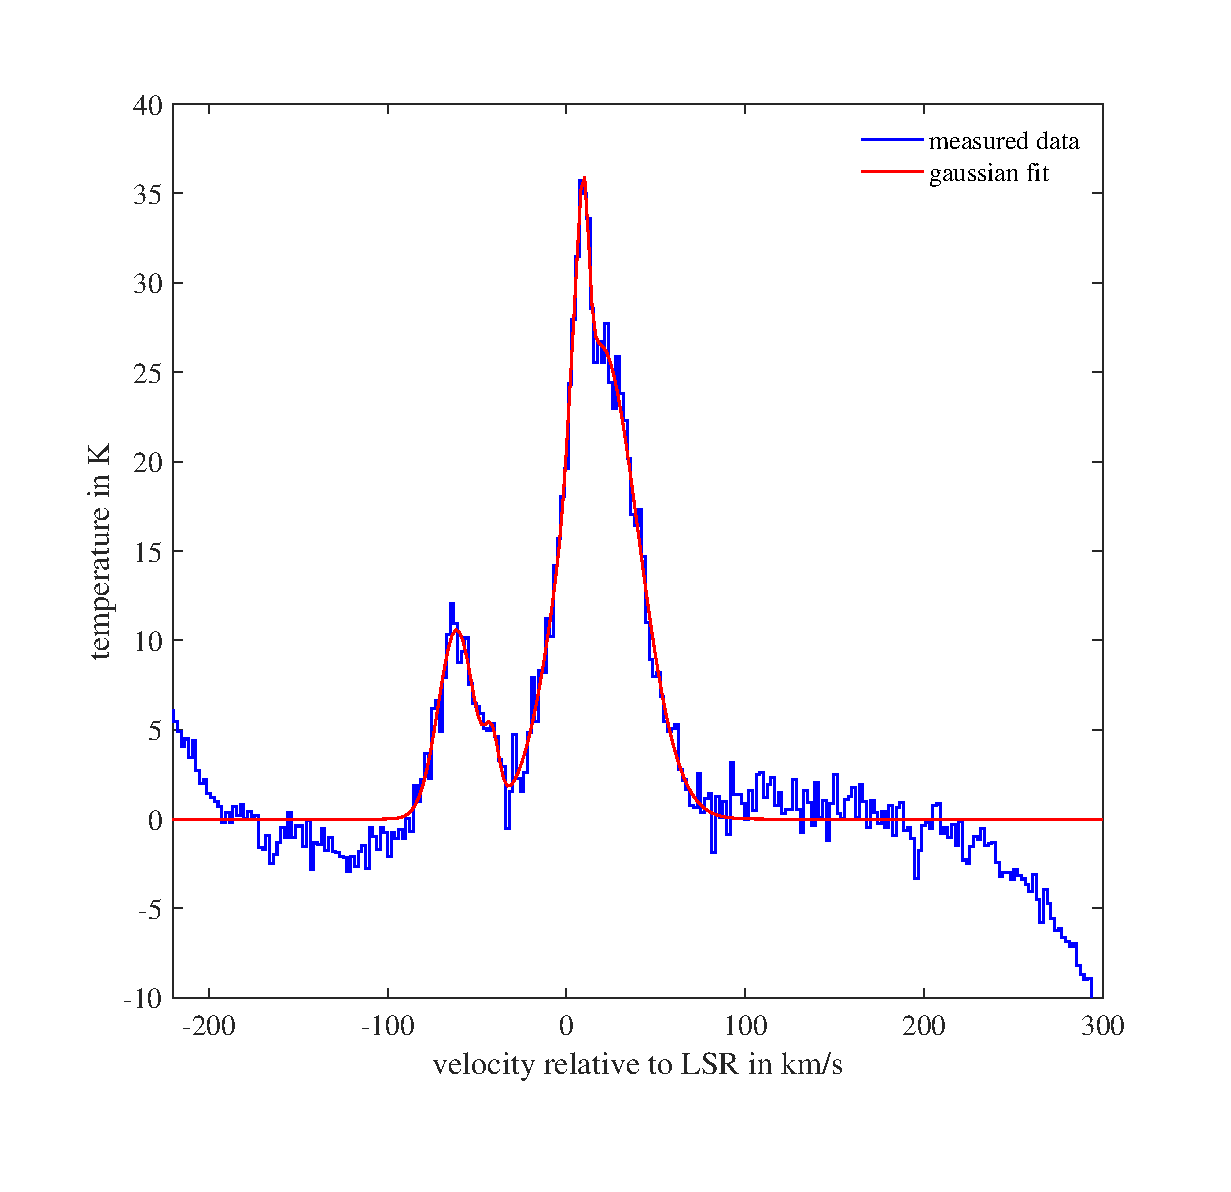
\includegraphics[width= 0.9\textwidth]{plots/TestBaseline.eps}
    \caption[Gemessenes Beispielspektrum zur Darstellung der Verarbeitung der Daten]{Gemessenes Beispielspektrum zur Darstellung der Verarbeitung der Daten. Da bei den Messungen stets ein Untergrundrauschen mitgemessen wird, muss dieses mithilfe eines Computerprogramms herausgefiltert werden. Mithilfe eines MatLab-Skripts sind die Spektren jeweils noch mit Gaußfunktionen gefittet. So lassen sich die Maxima deutlich erkennen und auslesen. In diesem Fall handelt es sich um eine Messung bei $l = \SI{30}{\degree}, \, b = \SI{0}{\degree}$ und die beiden Maxima liegen bei \SI{7.3}{\frac{km}{s}} und \SI{-64.8}{\frac{km}{s}} relativ zu LSR.}
    \label{fig:TestBaseline}
\end{figure}

\begin{figure}[H]
    \centering
    % GNUPLOT: LaTeX picture with Postscript
\begingroup
  % Encoding inside the plot.  In the header of your document, this encoding
  % should to defined, e.g., by using
  % \usepackage[cp1252,<other encodings>]{inputenc}
  \inputencoding{cp1252}%
  \makeatletter
  \providecommand\color[2][]{%
    \GenericError{(gnuplot) \space\space\space\@spaces}{%
      Package color not loaded in conjunction with
      terminal option `colourtext'%
    }{See the gnuplot documentation for explanation.%
    }{Either use 'blacktext' in gnuplot or load the package
      color.sty in LaTeX.}%
    \renewcommand\color[2][]{}%
  }%
  \providecommand\includegraphics[2][]{%
    \GenericError{(gnuplot) \space\space\space\@spaces}{%
      Package graphicx or graphics not loaded%
    }{See the gnuplot documentation for explanation.%
    }{The gnuplot epslatex terminal needs graphicx.sty or graphics.sty.}%
    \renewcommand\includegraphics[2][]{}%
  }%
  \providecommand\rotatebox[2]{#2}%
  \@ifundefined{ifGPcolor}{%
    \newif\ifGPcolor
    \GPcolorfalse
  }{}%
  \@ifundefined{ifGPblacktext}{%
    \newif\ifGPblacktext
    \GPblacktexttrue
  }{}%
  % define a \g@addto@macro without @ in the name:
  \let\gplgaddtomacro\g@addto@macro
  % define empty templates for all commands taking text:
  \gdef\gplbacktext{}%
  \gdef\gplfronttext{}%
  \makeatother
  \ifGPblacktext
    % no textcolor at all
    \def\colorrgb#1{}%
    \def\colorgray#1{}%
  \else
    % gray or color?
    \ifGPcolor
      \def\colorrgb#1{\color[rgb]{#1}}%
      \def\colorgray#1{\color[gray]{#1}}%
      \expandafter\def\csname LTw\endcsname{\color{white}}%
      \expandafter\def\csname LTb\endcsname{\color{black}}%
      \expandafter\def\csname LTa\endcsname{\color{black}}%
      \expandafter\def\csname LT0\endcsname{\color[rgb]{1,0,0}}%
      \expandafter\def\csname LT1\endcsname{\color[rgb]{0,1,0}}%
      \expandafter\def\csname LT2\endcsname{\color[rgb]{0,0,1}}%
      \expandafter\def\csname LT3\endcsname{\color[rgb]{1,0,1}}%
      \expandafter\def\csname LT4\endcsname{\color[rgb]{0,1,1}}%
      \expandafter\def\csname LT5\endcsname{\color[rgb]{1,1,0}}%
      \expandafter\def\csname LT6\endcsname{\color[rgb]{0,0,0}}%
      \expandafter\def\csname LT7\endcsname{\color[rgb]{1,0.3,0}}%
      \expandafter\def\csname LT8\endcsname{\color[rgb]{0.5,0.5,0.5}}%
    \else
      % gray
      \def\colorrgb#1{\color{black}}%
      \def\colorgray#1{\color[gray]{#1}}%
      \expandafter\def\csname LTw\endcsname{\color{white}}%
      \expandafter\def\csname LTb\endcsname{\color{black}}%
      \expandafter\def\csname LTa\endcsname{\color{black}}%
      \expandafter\def\csname LT0\endcsname{\color{black}}%
      \expandafter\def\csname LT1\endcsname{\color{black}}%
      \expandafter\def\csname LT2\endcsname{\color{black}}%
      \expandafter\def\csname LT3\endcsname{\color{black}}%
      \expandafter\def\csname LT4\endcsname{\color{black}}%
      \expandafter\def\csname LT5\endcsname{\color{black}}%
      \expandafter\def\csname LT6\endcsname{\color{black}}%
      \expandafter\def\csname LT7\endcsname{\color{black}}%
      \expandafter\def\csname LT8\endcsname{\color{black}}%
    \fi
  \fi
    \setlength{\unitlength}{0.0500bp}%
    \ifx\gptboxheight\undefined%
      \newlength{\gptboxheight}%
      \newlength{\gptboxwidth}%
      \newsavebox{\gptboxtext}%
    \fi%
    \setlength{\fboxrule}{0.5pt}%
    \setlength{\fboxsep}{1pt}%
\begin{picture}(7200.00,5040.00)%
    \gplgaddtomacro\gplbacktext{%
      \csname LTb\endcsname%%
      \put(814,704){\makebox(0,0)[r]{\strut{}$0$}}%
      \put(814,1561){\makebox(0,0)[r]{\strut{}$50$}}%
      \put(814,2419){\makebox(0,0)[r]{\strut{}$100$}}%
      \put(814,3276){\makebox(0,0)[r]{\strut{}$150$}}%
      \put(814,4133){\makebox(0,0)[r]{\strut{}$200$}}%
      \put(946,484){\makebox(0,0){\strut{}$4.5$}}%
      \put(1678,484){\makebox(0,0){\strut{}$5$}}%
      \put(2410,484){\makebox(0,0){\strut{}$5.5$}}%
      \put(3142,484){\makebox(0,0){\strut{}$6$}}%
      \put(3875,484){\makebox(0,0){\strut{}$6.5$}}%
      \put(4607,484){\makebox(0,0){\strut{}$7$}}%
      \put(5339,484){\makebox(0,0){\strut{}$7.5$}}%
      \put(6071,484){\makebox(0,0){\strut{}$8$}}%
      \put(6803,484){\makebox(0,0){\strut{}$8.5$}}%
    }%
    \gplgaddtomacro\gplfronttext{%
      \csname LTb\endcsname%%
      \put(209,2761){\rotatebox{-270}{\makebox(0,0){\strut{}V(R) in $\si{}{\frac{km}{s}}$}}}%
      \put(3874,154){\makebox(0,0){\strut{}Bahnradius in $\si{}{pc}$}}%
      \csname LTb\endcsname%%
      \put(5816,4646){\makebox(0,0)[r]{\strut{}constant velocity}}%
      \csname LTb\endcsname%%
      \put(5816,4426){\makebox(0,0)[r]{\strut{}linear fit}}%
    }%
    \gplbacktext
    \put(0,0){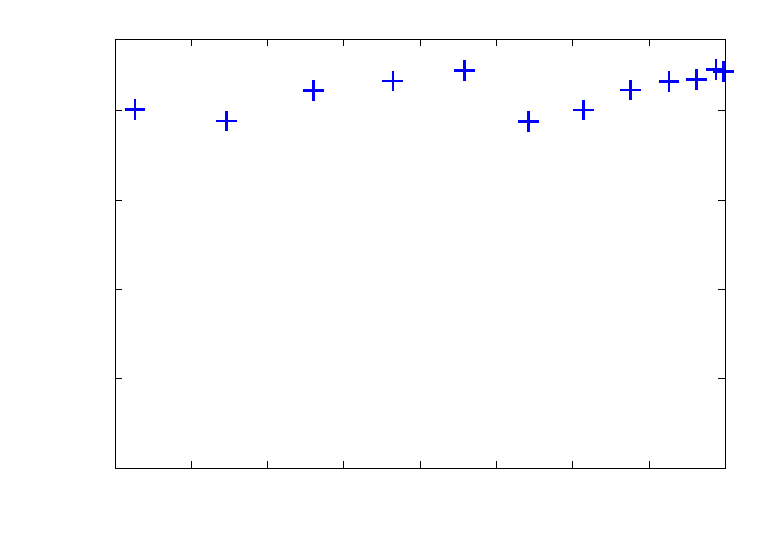
\includegraphics{plots/VvonR}}%
    \gplfronttext
  \end{picture}%
\endgroup

    \caption[Rotationskurve der Milchstraße]{Dargestellt ist eine Rotationskurve der Milchstraße. Die eingetragenen Datenpunkte sind jeweils aus dem Peak der maximal verschobenen Geschwindigkeitskomponente der gemessenen Geschwindigkeitsspekra aus dem ersten Quadranten gewonnen. Es ist deutlich zu erkennen, dass die Geschwindigkeit $V(R)$ nahezu unabhängig von dem Bahnradius ist. Mit einem linearen fit ist dies in der Abbildung nochmals verdeutlicht. Der Ordinatenabschnitt kennzeichnet dabei den Mittelwert der gemessenen Geschwindigkeiten. Dieser beträgt $\SI{210.9 \pm 3.1}{\frac{km}{s}}$ und kommt dem einem Literaturwert von $\SI{220}{\frac{km}{s}}$ \cite{LSR} sehr nahe. Einen exakten Literaturwert für die Geschwindigkeit zu finden ist nicht möglich, da dieser bei verschiedenen Quellen unterschiedlich angegeben wird. Jedoch wird immer ein Wert um $\SI{220}{\frac{km}{s}}$ angegeben.}
    \label{fig:VvonR}
\end{figure}
Da es im ersten Quadranten mehrere positive Lösungen für $r$ gibt, muss eine genauere Untersuchung der Beobachtungsrichtung gemacht werden. Hierfür werden
\begin{figure}[H]
    \centering
    % GNUPLOT: LaTeX picture with Postscript
\begingroup
  % Encoding inside the plot.  In the header of your document, this encoding
  % should to defined, e.g., by using
  % \usepackage[cp1252,<other encodings>]{inputenc}
  \inputencoding{cp1252}%
  \makeatletter
  \providecommand\color[2][]{%
    \GenericError{(gnuplot) \space\space\space\@spaces}{%
      Package color not loaded in conjunction with
      terminal option `colourtext'%
    }{See the gnuplot documentation for explanation.%
    }{Either use 'blacktext' in gnuplot or load the package
      color.sty in LaTeX.}%
    \renewcommand\color[2][]{}%
  }%
  \providecommand\includegraphics[2][]{%
    \GenericError{(gnuplot) \space\space\space\@spaces}{%
      Package graphicx or graphics not loaded%
    }{See the gnuplot documentation for explanation.%
    }{The gnuplot epslatex terminal needs graphicx.sty or graphics.sty.}%
    \renewcommand\includegraphics[2][]{}%
  }%
  \providecommand\rotatebox[2]{#2}%
  \@ifundefined{ifGPcolor}{%
    \newif\ifGPcolor
    \GPcolorfalse
  }{}%
  \@ifundefined{ifGPblacktext}{%
    \newif\ifGPblacktext
    \GPblacktexttrue
  }{}%
  % define a \g@addto@macro without @ in the name:
  \let\gplgaddtomacro\g@addto@macro
  % define empty templates for all commands taking text:
  \gdef\gplbacktext{}%
  \gdef\gplfronttext{}%
  \makeatother
  \ifGPblacktext
    % no textcolor at all
    \def\colorrgb#1{}%
    \def\colorgray#1{}%
  \else
    % gray or color?
    \ifGPcolor
      \def\colorrgb#1{\color[rgb]{#1}}%
      \def\colorgray#1{\color[gray]{#1}}%
      \expandafter\def\csname LTw\endcsname{\color{white}}%
      \expandafter\def\csname LTb\endcsname{\color{black}}%
      \expandafter\def\csname LTa\endcsname{\color{black}}%
      \expandafter\def\csname LT0\endcsname{\color[rgb]{1,0,0}}%
      \expandafter\def\csname LT1\endcsname{\color[rgb]{0,1,0}}%
      \expandafter\def\csname LT2\endcsname{\color[rgb]{0,0,1}}%
      \expandafter\def\csname LT3\endcsname{\color[rgb]{1,0,1}}%
      \expandafter\def\csname LT4\endcsname{\color[rgb]{0,1,1}}%
      \expandafter\def\csname LT5\endcsname{\color[rgb]{1,1,0}}%
      \expandafter\def\csname LT6\endcsname{\color[rgb]{0,0,0}}%
      \expandafter\def\csname LT7\endcsname{\color[rgb]{1,0.3,0}}%
      \expandafter\def\csname LT8\endcsname{\color[rgb]{0.5,0.5,0.5}}%
    \else
      % gray
      \def\colorrgb#1{\color{black}}%
      \def\colorgray#1{\color[gray]{#1}}%
      \expandafter\def\csname LTw\endcsname{\color{white}}%
      \expandafter\def\csname LTb\endcsname{\color{black}}%
      \expandafter\def\csname LTa\endcsname{\color{black}}%
      \expandafter\def\csname LT0\endcsname{\color{black}}%
      \expandafter\def\csname LT1\endcsname{\color{black}}%
      \expandafter\def\csname LT2\endcsname{\color{black}}%
      \expandafter\def\csname LT3\endcsname{\color{black}}%
      \expandafter\def\csname LT4\endcsname{\color{black}}%
      \expandafter\def\csname LT5\endcsname{\color{black}}%
      \expandafter\def\csname LT6\endcsname{\color{black}}%
      \expandafter\def\csname LT7\endcsname{\color{black}}%
      \expandafter\def\csname LT8\endcsname{\color{black}}%
    \fi
  \fi
    \setlength{\unitlength}{0.0500bp}%
    \ifx\gptboxheight\undefined%
      \newlength{\gptboxheight}%
      \newlength{\gptboxwidth}%
      \newsavebox{\gptboxtext}%
    \fi%
    \setlength{\fboxrule}{0.5pt}%
    \setlength{\fboxsep}{1pt}%
\begin{picture}(7200.00,5040.00)%
    \gplgaddtomacro\gplbacktext{%
      \csname LTb\endcsname%%
      \put(814,704){\makebox(0,0)[r]{\strut{}$-10$}}%
      \put(814,1292){\makebox(0,0)[r]{\strut{}$0$}}%
      \put(814,1880){\makebox(0,0)[r]{\strut{}$10$}}%
      \put(814,2468){\makebox(0,0)[r]{\strut{}$20$}}%
      \put(814,3055){\makebox(0,0)[r]{\strut{}$30$}}%
      \put(814,3643){\makebox(0,0)[r]{\strut{}$40$}}%
      \put(814,4231){\makebox(0,0)[r]{\strut{}$50$}}%
      \put(814,4819){\makebox(0,0)[r]{\strut{}$60$}}%
      \put(1191,484){\makebox(0,0){\strut{}$-200$}}%
      \put(2304,484){\makebox(0,0){\strut{}$-100$}}%
      \put(3418,484){\makebox(0,0){\strut{}$0$}}%
      \put(4531,484){\makebox(0,0){\strut{}$100$}}%
      \put(5645,484){\makebox(0,0){\strut{}$200$}}%
      \put(6758,484){\makebox(0,0){\strut{}$300$}}%
    }%
    \gplgaddtomacro\gplfronttext{%
      \csname LTb\endcsname%%
      \put(308,2761){\rotatebox{-270}{\makebox(0,0){\strut{}Temperatur in K}}}%
      \put(3874,154){\makebox(0,0){\strut{}Geschwindigkeit relativ zu LSR in $\frac{\text{km}}{\text{s}}$}}%
      \csname LTb\endcsname%%
      \put(5816,4646){\makebox(0,0)[r]{\strut{}$l = \si{78}{\degree}, b = \, \, \, \, \, \si{0}{\degree}$}}%
      \csname LTb\endcsname%%
      \put(5816,4426){\makebox(0,0)[r]{\strut{}$l = \si{78}{\degree}, b = \si{-2}{\degree}$}}%
      \csname LTb\endcsname%%
      \put(5816,4206){\makebox(0,0)[r]{\strut{}$l = \si{78}{\degree}, b = \, \, \, \, \, \si{2}{\degree}$}}%
    }%
    \gplbacktext
    \put(0,0){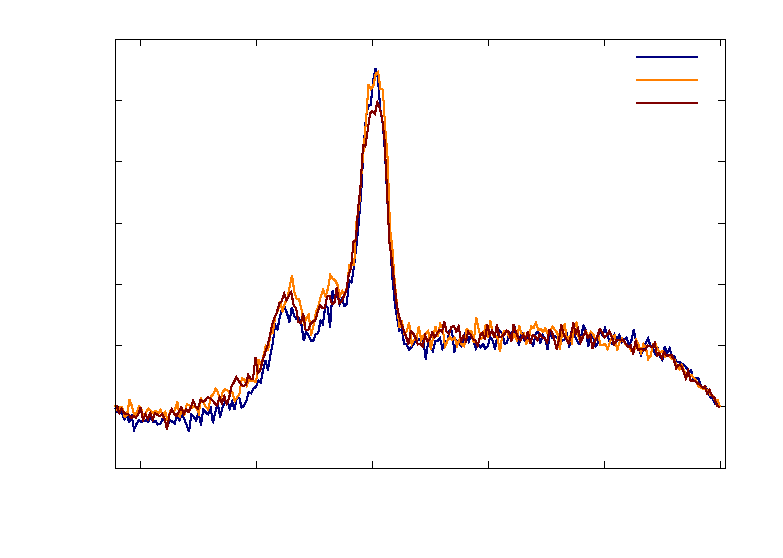
\includegraphics{plots/bungleichnull}}%
    \gplfronttext
  \end{picture}%
\endgroup
   
    \caption[Spektren für verschiedene galaktische Breiten $b$]{Spektren für verschiedene galaktische Breiten $b$. Erkennbar ist, dass bei den Spektren stets bei allen gewählten galaktische Breiten $b$ die Maxima bei \SI{2.4}{\frac{km}{s}}, \SI{-30.6}{\frac{km}{s}} und bei \SI{-69.7}{\frac{km}{s}} erkennbar sind. Die gewählten galaktischen Breiten sind also zu klein gewählt worden. Bei größeren galaktischen Breiten sollte dann mindestens ein Peak verschwinden. Auf die gefitteten Gaußkurven wurde bei dieser Abbildung aus Gründen der Lesbarkeit verzichtet.}
    \label{fig:bungleichnull}
\end{figure}

\begin{figure}[H]
    \centering
    % GNUPLOT: LaTeX picture with Postscript
\begingroup
  % Encoding inside the plot.  In the header of your document, this encoding
  % should to defined, e.g., by using
  % \usepackage[cp1252,<other encodings>]{inputenc}
  \inputencoding{cp1252}%
  \makeatletter
  \providecommand\color[2][]{%
    \GenericError{(gnuplot) \space\space\space\@spaces}{%
      Package color not loaded in conjunction with
      terminal option `colourtext'%
    }{See the gnuplot documentation for explanation.%
    }{Either use 'blacktext' in gnuplot or load the package
      color.sty in LaTeX.}%
    \renewcommand\color[2][]{}%
  }%
  \providecommand\includegraphics[2][]{%
    \GenericError{(gnuplot) \space\space\space\@spaces}{%
      Package graphicx or graphics not loaded%
    }{See the gnuplot documentation for explanation.%
    }{The gnuplot epslatex terminal needs graphicx.sty or graphics.sty.}%
    \renewcommand\includegraphics[2][]{}%
  }%
  \providecommand\rotatebox[2]{#2}%
  \@ifundefined{ifGPcolor}{%
    \newif\ifGPcolor
    \GPcolorfalse
  }{}%
  \@ifundefined{ifGPblacktext}{%
    \newif\ifGPblacktext
    \GPblacktexttrue
  }{}%
  % define a \g@addto@macro without @ in the name:
  \let\gplgaddtomacro\g@addto@macro
  % define empty templates for all commands taking text:
  \gdef\gplbacktext{}%
  \gdef\gplfronttext{}%
  \makeatother
  \ifGPblacktext
    % no textcolor at all
    \def\colorrgb#1{}%
    \def\colorgray#1{}%
  \else
    % gray or color?
    \ifGPcolor
      \def\colorrgb#1{\color[rgb]{#1}}%
      \def\colorgray#1{\color[gray]{#1}}%
      \expandafter\def\csname LTw\endcsname{\color{white}}%
      \expandafter\def\csname LTb\endcsname{\color{black}}%
      \expandafter\def\csname LTa\endcsname{\color{black}}%
      \expandafter\def\csname LT0\endcsname{\color[rgb]{1,0,0}}%
      \expandafter\def\csname LT1\endcsname{\color[rgb]{0,1,0}}%
      \expandafter\def\csname LT2\endcsname{\color[rgb]{0,0,1}}%
      \expandafter\def\csname LT3\endcsname{\color[rgb]{1,0,1}}%
      \expandafter\def\csname LT4\endcsname{\color[rgb]{0,1,1}}%
      \expandafter\def\csname LT5\endcsname{\color[rgb]{1,1,0}}%
      \expandafter\def\csname LT6\endcsname{\color[rgb]{0,0,0}}%
      \expandafter\def\csname LT7\endcsname{\color[rgb]{1,0.3,0}}%
      \expandafter\def\csname LT8\endcsname{\color[rgb]{0.5,0.5,0.5}}%
    \else
      % gray
      \def\colorrgb#1{\color{black}}%
      \def\colorgray#1{\color[gray]{#1}}%
      \expandafter\def\csname LTw\endcsname{\color{white}}%
      \expandafter\def\csname LTb\endcsname{\color{black}}%
      \expandafter\def\csname LTa\endcsname{\color{black}}%
      \expandafter\def\csname LT0\endcsname{\color{black}}%
      \expandafter\def\csname LT1\endcsname{\color{black}}%
      \expandafter\def\csname LT2\endcsname{\color{black}}%
      \expandafter\def\csname LT3\endcsname{\color{black}}%
      \expandafter\def\csname LT4\endcsname{\color{black}}%
      \expandafter\def\csname LT5\endcsname{\color{black}}%
      \expandafter\def\csname LT6\endcsname{\color{black}}%
      \expandafter\def\csname LT7\endcsname{\color{black}}%
      \expandafter\def\csname LT8\endcsname{\color{black}}%
    \fi
  \fi
    \setlength{\unitlength}{0.0500bp}%
    \ifx\gptboxheight\undefined%
      \newlength{\gptboxheight}%
      \newlength{\gptboxwidth}%
      \newsavebox{\gptboxtext}%
    \fi%
    \setlength{\fboxrule}{0.5pt}%
    \setlength{\fboxsep}{1pt}%
\begin{picture}(7200.00,5040.00)%
    \gplgaddtomacro\gplbacktext{%
      \csname LTb\endcsname%%
      \put(814,704){\makebox(0,0)[r]{\strut{}$-20$}}%
      \put(814,1218){\makebox(0,0)[r]{\strut{}$-15$}}%
      \put(814,1733){\makebox(0,0)[r]{\strut{}$-10$}}%
      \put(814,2247){\makebox(0,0)[r]{\strut{}$-5$}}%
      \put(814,2762){\makebox(0,0)[r]{\strut{}$0$}}%
      \put(814,3276){\makebox(0,0)[r]{\strut{}$5$}}%
      \put(814,3790){\makebox(0,0)[r]{\strut{}$10$}}%
      \put(814,4305){\makebox(0,0)[r]{\strut{}$15$}}%
      \put(814,4819){\makebox(0,0)[r]{\strut{}$20$}}%
      \put(946,484){\makebox(0,0){\strut{}$-20$}}%
      \put(1678,484){\makebox(0,0){\strut{}$-15$}}%
      \put(2410,484){\makebox(0,0){\strut{}$-10$}}%
      \put(3142,484){\makebox(0,0){\strut{}$-5$}}%
      \put(3875,484){\makebox(0,0){\strut{}$0$}}%
      \put(4607,484){\makebox(0,0){\strut{}$5$}}%
      \put(5339,484){\makebox(0,0){\strut{}$10$}}%
      \put(6071,484){\makebox(0,0){\strut{}$15$}}%
      \put(6803,484){\makebox(0,0){\strut{}$20$}}%
    }%
    \gplgaddtomacro\gplfronttext{%
      \csname LTb\endcsname%%
      \put(209,2761){\rotatebox{-270}{\makebox(0,0){\strut{}y in $\si{}{pc}$}}}%
      \put(3874,154){\makebox(0,0){\strut{}x in $\si{}{pc}$}}%
    }%
    \gplbacktext
    \put(0,0){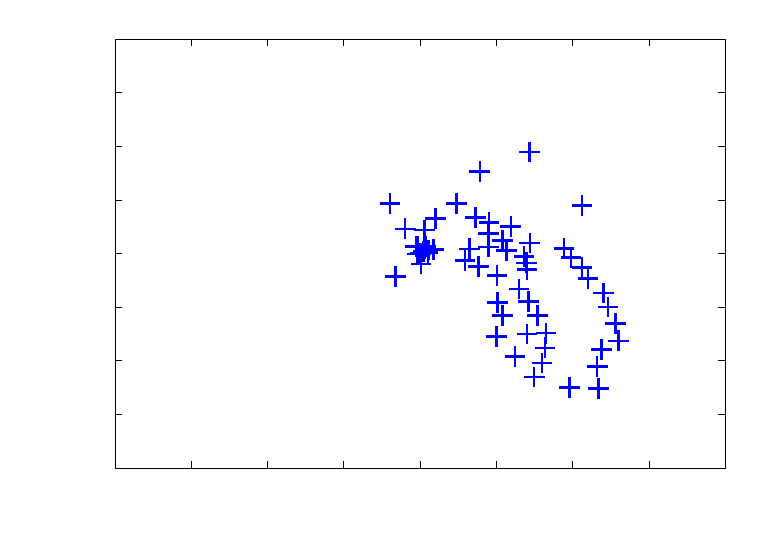
\includegraphics{plots/Milchstrassesafe}}%
    \gplfronttext
  \end{picture}%
\endgroup
   
    \caption[Abbildung der Milchstraße]{In dieser Abbildung ist die Milchstraße mithilfe der Daten aus den Frequenzspektra katografiert. Bei der Abbildung ist ein Seitenarme der Milchstraße im Bereich um $(x,y)=(10,-10)$ deutlich ersichtlich. Ein weiterer Galaxiearm ist im Bereich $(x,y)=(10,5)$ erkennbar, wobei dieser schon deutlich schwächer ausgeprägt ist. In dem Bereich um den Ursprung sind die Datenpunkte sehr dicht angehäuft. Somit ist in diesem Bereich leider keine eindeutige Aussage über etwaige Galaxiearme treffbar. Mithilfe des eingefärbten Kreises mit dem Radius von $\si{25}{kpc}$ ist die größe der gesamten Galxie ersichtlich.}
    \label{fig:Milchstrassesafe}
\end{figure}



